\documentclass[11pt]{article}
\usepackage[margin=1in]{geometry}
\usepackage[T1]{fontenc}
\usepackage{lmodern}
\usepackage{amsmath,amssymb,mathtools,booktabs}
\usepackage{graphicx}
\usepackage{hyperref}
\usepackage[numbers,sort&compress]{natbib}
\setlength{\emergencystretch}{2em}

\title{Boundary-Mode Topographic Cosmology:\\
A Reduced-Response Bridge from Berger--Hopf Geometry to Late-Time Structure Growth}
\author{Norman P. Carberry\\Independent Researcher}
\date{Working draft --- September 2026}

\newcommand{\Mpl}{M_{\rm Pl}}
\newcommand{\OmK}{\Omega_k}
\newcommand{\RH}{R_H}
\newcommand{\Kphys}{\mathcal K_{\rm phys}}

\begin{document}
\maketitle

\begin{abstract}
We develop a late-time cosmological bridge between a scalar topographic effective field theory on compact spatial sections \(S^3(R_H)\) and the constraint-reduced response architecture of the Berger--Hopf program. The construction keeps a covariant cubic-Galileon background with second-order time evolution and introduces the higher-spatial-gradient response as the low-energy Schur/Feshbach reduction of a stable physical complement rather than as a fundamental higher-time-derivative interaction. On \(S^3\), scalar harmonics obey \(-\nabla^2Y_n=n(n+2)Y_n/R_H^2\). The reduced response can therefore soften the lowest nonconstant \(n=1\) branch while stiffening \(n\ge2\), providing a mechanism for a large low-redshift dipolar susceptibility without a comparable quadrupole or large modification of ordinary redshift-space-distortion modes. We define a reference branch R1, specify an auditable preregistration protocol, and derive prospective growth and lensing targets. The low-redshift supernova amplitude is used only as an observational normalization of the \(n=1\) response; the curvature forecast and structure-growth predictions are kept logically separate. The framework is explicitly falsifiable through spatial curvature, harmonic hierarchy, fixed-axis anisotropy, growth, and lensing tests.
\end{abstract}

\section{Introduction}

Late-time cosmological tensions and directional residuals motivate tests that are capable of separating local structure, survey geometry, and genuinely new large-scale dynamics. The scalar-topographic program introduced a compact hyperspherical parent \(S^3(R_H)\) and a long-wavelength scalar response whose largest observational effect occurs at low redshift \citep{Carberry2026Topographic}. A later covariant formulation placed the topographic scalar in the cubic-Galileon sector of Horndeski theory, preserving second-order time evolution while allowing nontrivial late-time scalar--metric braiding.

The present work asks a narrower question: can the long-wavelength topographic response be represented as the large-scale branch of the same constraint-reduced response logic used in the Berger--Hopf program, without assuming that the full microscopic BHSM construction has already been compactified into cosmology? We answer this at the level of a controlled bridge model.

The central mathematical chain is
\[
S[\Phi]
\longrightarrow
\widehat{\mathcal H}_{\rm phys}
\longrightarrow
\mathcal K_{\rm topo}
\longrightarrow
\lambda_{\rm topo}
\longrightarrow
T_n
\longrightarrow
\delta g_{\mu\nu}
\longrightarrow
\{D_L,H,f\sigma_8,\Phi+\Psi\}.
\]

The distinction between established input and bridge extension is essential. The \(S^3\) harmonic spectrum and cubic-Galileon background are treated as the cosmological starting point. The Schur/Feshbach reduction is an exact mathematical operation once a physical complement is specified. The identification of its low-energy coefficients with the topographic response is a bridge assumption to be tested, not a declaration that the complete microscopic BHSM action has already been reduced to four-dimensional cosmology.

The paper makes four main contributions. First, it standardizes the \(S^3\) harmonic convention and shows how the observed sky dipole arises from the four-dimensional \(n=1\) eigenspace rather than by identifying a radial mode with an angular dipole. Second, it derives a reduced kernel in which a positive higher-spatial-gradient term can emerge after integrating out a stable complement. Third, it identifies a parameter interval in which the \(n=1\) response is selectively softened while all \(n\ge2\) harmonics are stiffened. Fourth, it gives an executable preregistration protocol for curvature, supernova anisotropy, growth, and lensing tests.

The claim boundary is therefore:
\begin{quote}
This work does not assume that the scalar-topographic cosmological field has already been derived from the complete microscopic Berger--Hopf action. Exact reductions are distinguished from cross-scale identifications and exploratory reference-branch assumptions. Prospective observables are frozen before comparison with designated independent data.
\end{quote}


\section{Hyperspherical Parent and Harmonic Convention}

We use a closed FLRW geometry
\[
ds^2=-dt^2+a^2(t)R_H^2\left[d\psi^2+\sin^2\psi\,d\Omega_2^2\right],
\]
with \(a_0=1\). Here \(\psi\) is a dimensionless radial angle on the unit three-sphere, \(R_H\) is the present-day comoving curvature radius, and the physical curvature radius is \(aR_H\). To avoid mixing dimensional and angular radial coordinates, define
\[
D_C(z)=c\int_0^z\frac{dz'}{H(z')},
\qquad
\psi(z)=\frac{D_C(z)}{R_H}.
\]

Scalar harmonics satisfy
\[
-\nabla_\gamma^2Y_n=\frac{n(n+2)}{R_H^2}Y_n,
\qquad
n=0,1,2,\ldots,
\]
with degeneracy \((n+1)^2\). The physical spatial eigenvalue entering the time-dependent perturbation equations is
\[
p_n(a)=\frac{n(n+2)}{a^2R_H^2}.
\]

The first nonconstant eigenspace is therefore
\[
p_1=\frac{3}{a^2R_H^2}.
\]
This convention is used throughout. Older scalar-topographic notes employed more than one normalization for the lowest mode; no numerical forecast is carried forward here without first converting it to the convention above.

\subsection{Exact observer-sky form of the n=1 scalar mode}

Embed the unit three-sphere in \(\mathbb R^4\). The \(n=1\) scalar harmonics are the four coordinate functions restricted to \(S^3\). A general real \(n=1\) scalar mode can therefore be written
\[
T_1(\psi,\hat{\mathbf n})
=
A\left[
\cos\alpha\cos\psi
+
\sin\alpha\sin\psi\,
(\hat{\mathbf n}\cdot\hat{\mathbf p})
\right].
\]
At fixed radial shell this scalar function contains an exact sky monopole plus an exact sky dipole and no higher angular multipoles. Its dipolar part is
\[
T_{1,{\rm dip}}(z,\hat{\mathbf n})
=
A\sin\alpha\,
\sin\!\psi(z)\,
(\hat{\mathbf n}\cdot\hat{\mathbf p}).
\]
This removes an ambiguity present in simplified radial descriptions: the zonal term \(\cos\psi\) alone is isotropic for an observer at its pole. A sky dipole in the scalar field is supplied by a generic orientation of the full \(n=1\) eigenspace relative to the observer.

\subsection{Exceptional lowest scalar harmonic and metric-response caveat}

The existence of the scalar function above must be distinguished from its use as an ordinary scalar \emph{metric} perturbation of closed FLRW. A common closed-universe convention labels scalar eigenvalues as
\[
k^2=N^2-1,
\qquad N=1,2,3,\ldots
\]
for unit positive curvature. Our convention \(n(n+2)\) is related by
\[
N=n+1.
\]
Thus our first nonconstant \(n=1\) scalar level maps to \(N=2\) in that literature.

Gauge-invariant closed-FLRW perturbation constructions contain factors such as
\[
\frac{1}{N^2-4\mathcal K},
\]
which are singular at \(N=2\) for \(\mathcal K=+1\), and the usual scalar-derived tensor-harmonic construction treats the lowest \(N=1,2\) sectors as exceptional \citep{KieferVardanyan2022}. This does not remove the \(S^3\) scalar eigenfunction itself. It means that the ordinary metric-perturbation construction degenerates precisely at the harmonic level used here.

Accordingly, the monopole-plus-dipole result above is an exact statement about the topographic scalar pattern. A physical luminosity-distance, velocity, or gravitational-potential dipole does \emph{not} follow from that geometry alone. The bridge requires a separate constrained, gauge-invariant derivation of the scalar--metric response in this exceptional sector. Until that calculation is supplied, every metric or light-cone prediction sourced by the \(n=1\) field is conditional on this consistency requirement.

\section{Constraint-Reduced Response and the Topographic Kernel}

Let \(\widehat{\mathcal H}\) be the physical Hessian after constraints and gauge directions have been removed. For a selected topographic branch \(P\) and physical complement \(Q\), the exact Schur/Feshbach reduced operator is
\[
\mathcal K
=
P\left[
\widehat{\mathcal H}
-
\widehat{\mathcal H}Q
(Q\widehat{\mathcal H}Q)^{-1}
Q\widehat{\mathcal H}
\right]P.
\]

For one scalar harmonic, write the quadratic block as
\[
\widehat{\mathcal H}_n
=
\begin{pmatrix}
A(p) & C(p)\\
C^\dagger(p) & D(p)
\end{pmatrix}.
\]
The exact reduced stiffness is
\[
K_{\rm red}(p)=A(p)-C(p)D^{-1}(p)C^\dagger(p).
\]

A minimal long-wavelength realization is
\[
A(p)=Z_0p,\qquad
D(p)=M_c^2+c_cp,\qquad
C(p)=g\sqrt p.
\]
Then
\[
K_{\rm red}(p)
=
Z_0p-\frac{g^2p}{M_c^2+c_cp}.
\]
For \(c_cp\ll M_c^2\),
\[
K_{\rm red}(p)
=
\left(Z_0-\frac{g^2}{M_c^2}\right)p
+
\frac{g^2c_c}{M_c^4}p^2
+O(p^3).
\]

Thus a positive \(p^2\) stiffness can arise from a coupled second-order parent system after a stable complement is integrated out. In this interpretation the old static operator
\[
-\nabla^2+B\nabla^4
\]
is a low-energy spatial derivative expansion, not evidence for a fundamental fourth-order time equation.

Define
\[
\chi\equiv\frac{g^2}{M_c^2},
\qquad
L_c^2\equiv\frac{c_c}{M_c^2}.
\]
After canonical normalization of the leading spatial term, the reduced kernel may be written schematically as
\[
K_{\rm topo}(p)
=
m_T^2+
(c_s^2-\chi)p
+
\chi L_c^2p^2+\cdots.
\]
The signs of the temporal kinetic term and of the full physical gradient matrix must be checked independently; a positive spatial \(p^2\) coefficient by itself is not a complete ghost analysis.


\section{Cubic-Galileon Scalar--Metric Bridge}

The conditional R1 effective background action, used as a compatibility representation rather than a completed BHSM parent action, is taken to be
\[
S=
\int d^4x\sqrt{-g}
\left[
\frac{M_{\rm Pl}^2}{2}R
-\frac12\nabla_\mu T\nabla^\mu T
+\frac{1}{\Lambda^3}\Box T(\nabla T)^2
-V(T)
+\mathcal L_m
\right].
\]
Using
\[
X\equiv-\frac12\nabla_\mu T\nabla^\mu T,
\]
this corresponds to
\[
G_2=X-V(T),\qquad
G_3=\frac{2X}{\Lambda^3},\qquad
G_4=\frac{M_{\rm Pl}^2}{2},\qquad
G_5=0
\]
in the convention \(\mathcal L_3=-G_3\Box T\).

The model belongs to the kinetic-gravity-braiding subclass of Horndeski theory \citep{DeffayetKGB2010,BelliniSawicki2014}. Since \(G_4\) is constant and \(G_5=0\),
\[
M_*^2=M_{\rm Pl}^2,\qquad
\alpha_M=0,\qquad
\alpha_T=0.
\]
The scalar--metric mixing is controlled by the braiding function
\[
\alpha_B
=
\frac{2\dot{\bar T}^{\,3}}
{HM_{\rm Pl}^2\Lambda^3},
\]
and
\[
\alpha_K
=
\frac{\dot{\bar T}^{\,2}}
{H^2M_{\rm Pl}^2}
+
6\alpha_B.
\]
In the Bellini--Sawicki organization of Horndeski perturbations the scalar kinetic combination is
\[
D_{\rm kin}
=
\alpha_K+\frac32\alpha_B^2.
\]
Their perturbation equations are formulated for a spatially flat background \citep{BelliniSawicki2014}. We therefore use \(D_{\rm kin}>0\) below as an inherited kinetic diagnostic for the cubic-Galileon sector, not as a complete proof of perturbative stability for the present closed background plus the additional reduced spatial response. A full stability proof requires the constrained gauge-invariant kinetic and gradient matrices, including the exceptional lowest scalar sector identified above.

For numerical work we softly break shift symmetry with
\[
V(T)=V_0-\mu^3T.
\]
The scalar energy density and pressure are
\[
\rho_T
=
\frac12\dot T^2+V(T)
+\frac{6H\dot T^3}{\Lambda^3},
\]
\[
P_T
=
\frac12\dot T^2-V(T)
-\frac{2\dot T^2\ddot T}{\Lambda^3}.
\]
The shift current
\[
J=\dot T+\frac{6H\dot T^2}{\Lambda^3}
\]
obeys
\[
\dot J+3HJ=\mu^3.
\]
These background expressions are the standard kinetic-gravity-braiding relations specialized to the present \(G_2,G_3\) choice \citep{DeffayetKGB2010}.

The closed-FLRW background equation is
\[
3M_{\rm Pl}^2
\left(
H^2+\frac{1}{a^2R_H^2}
\right)
=
\rho_m+\rho_r+\rho_T.
\]

The bridge does not require the bare Horndeski sound speed to become negative. Instead, the BHSM-inspired reduced response is used to lower the effective long-wavelength spatial stiffness while a positive \(p^2\) term stiffens shorter wavelengths. This statement concerns the reduced spatial kernel; it is not, by itself, a complete closed-FLRW stability theorem.


\section{Selective Harmonic Response}

Let the complement correlation length scale with the parent radius,
\[
L_c(a)=aR_H\,\ell,
\]
where \(\ell\) is dimensionless. Since
\[
p_n=\frac{n(n+2)}{a^2R_H^2},
\]
we have
\[
L_c^2p_n=\ell^2n(n+2).
\]

In the effectively massless topographic sector, define
\[
K_n=p_nC_n
\]
with
\[
\boxed{
C_n(a)
=
c_s^2(a)
-
\chi(a)\left[1-\ell^2n(n+2)\right].
}
\]

If
\[
\boxed{
\frac18<\ell^2<\frac13,
}
\]
then
\[
1-3\ell^2>0
\]
for \(n=1\), whereas
\[
1-\ell^2n(n+2)<0
\]
for every \(n\ge2\). Hence increasing \(\chi\) softens the \(n=1\) response but stiffens all higher \(S^3\) scalar levels:
\[
C_1<c_s^2,\qquad
C_n>c_s^2\quad(n\ge2).
\]

This defines a selective positive-kernel branch within the reduced spatial ansatz. If
\[
0<C_1\ll1,
\]
then a sourced mode
\[
T_1\simeq\frac{S_1}{p_1C_1}
\]
can be strongly enhanced while the \(n\ge2\) responses remain regular. This positivity statement is narrower than a full perturbative stability result because the complete closed-background kinetic/gradient system has not yet been diagonalized.

For the next \(S^3\) scalar level,
\[
\frac{T_2}{T_1}
=
\frac{S_2}{S_1}
\frac{3C_1}{8C_2},
\]
so the response per unit source satisfies
\[
\left|
\frac{T_2/S_2}{T_1/S_1}
\right|
=
\frac{3C_1}{8C_2}
<
\frac38
\]
on the positive selective-filter branch, with much stronger suppression as \(C_1/C_2\to0\).

This is an \(S^3\) harmonic-level null test, not directly a sky-quadrupole-to-dipole ratio. The \(n=2\) eigenspace can project onto several observer-sky angular multipoles; an observational \(\ell_{\rm sky}=2\) prediction requires the explicit observer-shell projection and source weights.


\section{Observable Projection}

The observable distance perturbation is not identified directly with the scalar amplitude. At linear order it is a light-cone projection of metric, velocity, and scalar perturbations:
\[
\frac{\delta D_L}{\bar D_L}
=
\int d\chi\,
\left[
W_\Phi\Phi+
W_\Psi\Psi+
W_vv_\parallel+\cdots
\right].
\]
If the selected \(n=2\) curvature-scale sector admits a physical gauge-invariant metric response, its exact scalar angular dependence can factor as
\[
\hat{\mathbf n}\cdot\hat{\mathbf p},
\]
leading schematically to
\[
\frac{\delta D_L}{\bar D_L}
=
\epsilon_D(z)\,
\hat{\mathbf n}\cdot\hat{\mathbf p}.
\]
The existence and normalization of \(\epsilon_D(z)\) are therefore bridge outputs to be derived, not consequences of the scalar harmonic geometry alone.

For supernovae,
\[
\mu=5\log_{10}D_L+\mathrm{const},
\]
and therefore a small magnitude dipole \(A_\mu\) corresponds to
\[
\frac{\delta D_L}{D_L}
=
\frac{\ln10}{5}A_\mu\cos\theta.
\]

For structure growth we define
\[
k^2\Psi
=
-4\pi Ga^2\mu(k,a)\rho_m\delta_m,
\qquad
\Phi=\gamma(k,a)\Psi,
\]
and
\[
\Sigma(k,a)
=
\frac{\mu(k,a)}2[1+\gamma(k,a)].
\]
The matter growth factor obeys
\[
D''+
\left(2+\frac{H'}H\right)D'
-\frac32\Omega_m(a)\mu(k,a)D=0,
\]
with prime denoting \(d/d\ln a\). The observable is
\[
f\sigma_8(k,z)
=
\frac{D'}{D}D\,\sigma_{8,\rm ini}
=
D'(k,z)\sigma_{8,\rm ini}.
\]

The quasi-static limit is used only on scales inside the scalar sound horizon \citep{SawickiBellini2015}. Horizon-scale \(n=2\) observables require the full constrained long-wavelength response and must not be obtained by extrapolating quasi-static formulas into the first physical curvature-scale mode.

% BEGIN R1_COSMOLOGY_CLOSURE_V15
\subsection{Current action-native observable status}
\label{sec:r1-observable-status-v15}

The present R1 observable construction is evaluated on the canonical
two-component state
\[
X_2=(q_2,\Pi_2),
\qquad
q_2=\zeta_{\rm anchor},
\qquad
\Pi_2=2a_{\rm anchor}^3\mathcal G_{S,2}\dot\zeta_{\rm anchor}.
\]
Legacy response rows expressed in $(\zeta,d\zeta/dN)$ coordinates are not
interchangeable with these canonical rows without the explicit basis
transformation.

For standard candles the action-native fixed-observed-redshift luminosity-distance
row is denoted $\mathcal F_{D_L}(z)$. Distance duality then closes the
transverse late-time BAO distance response,
\[
\boxed{\mathcal F_{D_M/r_d}(z)=\mathcal F_{D_L}(z)},
\qquad d\ln r_d=0.
\]
This statement concerns the observed distance to the standard ruler, not an
intrinsic deformation of the sound horizon.

The historical closed-background expansion
\[
\frac{\Delta r_{\rm BAO}}{r_{\rm BAO}}
\simeq -\frac{K\chi^2(z)}{6}
\]
is therefore retained only as a background distance-projection expression. For
the frozen R1 radius $R_H=33.153\,\mathrm{Gpc}$, curvature across a
$150\,\mathrm{Mpc}$ ruler itself would produce only
$-3.412e-06$ at leading order, whereas the Gpc-baseline projection
at $z=0.93$ is $-1.562e-03$.

The radial observable remains an explicit open kernel:
\[
\mathcal F_{D_H/r_d}(z)=-\mathcal F_H(z)
\]
on the same late-time branch. We do not promote a numerical derivative of the
transverse distance kernel to $\mathcal F_H$, because the transverse light-cone
response contains metric, velocity, and integrated optical terms that need not
reduce to a single radial remapping. Survey window and covariance projection
are downstream of these cosmic kernels.
% END R1_COSMOLOGY_CLOSURE_V15


\section{Predictions and Falsification Criteria}

\subsection{Low-redshift calibration}

The Pantheon+ data release and cosmological analysis provide the supernova basis for the carried-forward tomographic calibration used here \citep{Scolnic2022,Brout2022}. The earlier scalar-topographic analysis reported
\[
A_\mu^\star=-0.0412\pm0.009
\]
in the bin
\[
0.01<z<0.03,
\]
with best-fit direction
\[
({\rm RA},{\rm Dec})
=
(211.48^\circ,-12.81^\circ).
\]
This corresponds to
\[
\frac{\delta D_L}{D_L}
=
(-0.01895\pm0.00414)\cos\theta,
\]
and at sufficiently low redshift,
\[
\frac{\delta H}{H}
=
(+0.01895\pm0.00414)\cos\theta.
\]

These numbers retain the earlier exploratory calibration; its original
likelihood is not reconstructed here. Section~\ref{sec:sn-sightlines} instead
uses the separately frozen later full-covariance amplitude
$A=-0.04321623436$ mag. The two calibrations must not be conflated, and
neither is retuned by the new interpretation test. The historical numbers
normalize only the selected physical \(n=2\) response,
\[
A_\mu
=
\frac{\mathcal K_{\rm SN}S_2}{p_2C_2},
\]
and do not independently determine \(S_2\), \(\mathcal K_{\rm SN}\), or \(C_2\). The physical distance row is now explicit; one scalar calibration leaves a state-space null direction.

\subsection{Curvature}

The pre-existing prospective curvature forecast is retained without retuning:
\[
\boxed{\Omega_k=-0.018\pm0.004}.
\]
At \(H_0=67.4\ {\rm km\,s^{-1}\,Mpc^{-1}}\),
\[
R_H
=
\frac{c}{H_0\sqrt{|\Omega_k|}}
\simeq33.15\ {\rm Gpc}.
\]
The sign prediction is \(\Omega_k<0\) in the usual FLRW curvature convention.

This value is a frozen model forecast, not a current empirical best fit. DESI DR2 BAO results are reported as well described by flat \(\Lambda\)CDM, even while combinations with other probes motivate tests of extensions such as dynamical dark energy \citep{DESIDR2ResultsII2025}. The purpose of retaining \(-0.018\pm0.004\) is therefore prospective falsification: it must be compared against independent curvature inference without being moved toward the observed result.

\subsection{Harmonic hierarchy}

The retained illustrative harmonic-filter realization predicts selective \(n=2\) softening with no analogous \(n\ge3\) enhancement. A future source-normalized \(S^3\) \(n=3\) susceptibility comparable to or larger than the physical \(n=2\) susceptibility would reject the minimal harmonic-filter branch. This statement is made at the compact-space harmonic level; comparison to a measured sky quadrupole requires an explicit observer-shell projection.

\subsection{Fixed-axis test}

A prospective independent supernova sample should first test the carried-forward axis
\[
(211.48^\circ,-12.81^\circ)
\]
rather than scanning freely over the sky. A free-axis search may be reported secondarily.

\subsection{High-n recovery}

Within the retained illustrative polynomial filter, at large \(n\),
\[
C_n\simeq\chi\ell^2n^2,
\]
so the extra scalar susceptibility falls as \(n^{-2}\). This conditional filter realization therefore predicts a strong separation between the first physical compact-space level and conventional clustering modes.

\subsection{Failure conditions}

The specified conditional realization (including its illustrative filter for the harmonic and high-$n$ tests) is disfavored if one or more of the following are established with adequate precision:
\begin{enumerate}
\item independent curvature measurements exclude the frozen negative-\(\Omega_k\) forecast;
\item the source-normalized \(S^3\) \(n=3\) response is comparable to or exceeds physical \(n=2\);
\item an independent low-redshift sample excludes the frozen dipole axis while finding a stable incompatible physical axis;
\item a coherent metric/light-cone dipole of comparable amplitude persists into a redshift regime in which the completed model predicts loss of enhanced susceptibility;
\item ordinary RSD modes show a large scale-independent modification incompatible with the high-\(n\) suppression;
\item lensing requires a metric response incompatible with the same completed scalar--metric propagator that controls matter clustering;
\item the selected physical \(n=2\) response cannot satisfy the common-domain constraint or stability requirements.
\end{enumerate}

% BEGIN R1_COSMOLOGY_CLOSURE_V15


% BEGIN PRE_PEER_REVIEW_LEGACY_STATUS_V1
\subsection{Role of carried-forward phenomenology}
The numerical low-redshift supernova calibration, fixed axis, and historical
curvature amplitude entered this project before the present geometry-first
physical reduction.  They are retained here as frozen calibration or
prospective legacy forecasts against which the new constrained construction
can be tested; they do not define the physical $n=2$ state or its observable
kernels.  In particular, the closed $S^3$ parent fixes the sign
$\Omega_k<0$ in the adopted FLRW convention, whereas the numerical forecast
$\Omega_k=-0.018\pm0.004$ is a carried-forward model forecast rather than a
new action-native determination of $|\Omega_k|$.

The same distinction applies to BAO and growth.  The current action-native
transverse distance response satisfies
$\mathcal F_{D_M/r_d}=\mathcal F_{D_L}$ conditional on
$\delta\ln r_d=0$.  The exact radial kernel
$\mathcal F_{D_H/r_d}=-\mathcal F_H$ and the survey-window/covariance
projection needed for a publishable RSD or radial-BAO comparison remain open.
The historical direct BAO--SN amplitude proportionality is therefore retained
only as provenance, not as the final prediction object.
% END PRE_PEER_REVIEW_LEGACY_STATUS_V1

\subsection{Status of the historical BAO--SN proportionality}
\label{sec:r1-bao-sn-status-v15}

The historical phenomenological forecast
$\mathcal R_{\rm BS}\sim700$--$800\,
\mathrm{km\,s^{-1}\,Mpc^{-1}}$ is retained as part of the development
record, but it is not asserted here as a closed action-native coefficient.
The modern R1 realization propagates a two-component canonical state through
observable-specific kernels, so the final falsification test is a common-state
trajectory evaluated at explicit epochs and through the appropriate standard
candle, transverse-BAO, radial-BAO, growth, or lensing response.

The low-redshift supernova calibration is kept separate from the global
high-redshift state inference. At $z_\star=0.02$ the empirical
calibration corresponds to
\[
|\Delta H_0|=1.279\pm0.279\,
\mathrm{km\,s^{-1}\,Mpc^{-1}},
\]
whereas the present high-redshift canonical state propagated to the same
low-redshift point gives a central value
\[
|\Delta H_0|_{\rm global}=0.01017\,
\mathrm{km\,s^{-1}\,Mpc^{-1}}.
\]
Consequently the minimal homogeneous/global realization is not used as a
substitute for the local calibration. Any local/topographic contribution
needed to predict that amplitude must be modeled and tested separately; no
retuning of the frozen canonical state is performed here.

The currently closed prediction structure is therefore:
\[
X_2\longrightarrow
\left\{
\mathcal F_{D_L},
\mathcal F_{D_M/r_d},
\mathcal F_{\rm growth},
\mathcal F_{\rm Weyl}
\right\},
\]
with $\mathcal F_{D_H/r_d}=-\mathcal F_H$ and survey-specific BAO
pair-window/covariance projection remaining open. These open objects are
future falsification targets rather than quantities filled by surrogate
relations.
% END R1_COSMOLOGY_CLOSURE_V15

\section{Numerical Implementation and Preregistration Protocol}

The numerical pipeline is separated into
\[
\boxed{
\text{background}
\rightarrow
\text{physical scalar response}
\rightarrow
\text{observables}
\rightarrow
\text{comparison}.
}
\]
Prediction generation and data comparison are implemented in separate scripts.

\subsection{Background system}

Let \(v=\dot T\). Expanding the scalar current equation gives
\[
\left(1+\frac{12Hv}{\Lambda^3}\right)\dot v
+
\frac{6v^2}{\Lambda^3}\dot H
=
\mu^3-3H\left(v+\frac{6Hv^2}{\Lambda^3}\right).
\]
The Raychaudhuri equation gives
\[
\frac{2v^2}{\Lambda^3}\dot v
-
2M_{\rm Pl}^2\dot H
=
\rho_m+\frac43\rho_r+v^2+\frac{6Hv^3}{\Lambda^3}
-\frac{2M_{\rm Pl}^2}{a^2R_H^2}.
\]
At each integration step these equations form a \(2\times2\) linear system for \((\dot v,\dot H)\). The remaining equations are
\[
\dot T=v,\qquad
\dot a=aH.
\]

The Friedmann equation is retained as an independent residual check:
\[
3M_{\rm Pl}^2
\left(H^2+\frac{1}{a^2R_H^2}\right)
-
(\rho_m+\rho_r+\rho_T)
=0.
\]

\subsection{Dimensionless variables}

We integrate in \(N=\ln a\) with
\[
E=\frac{H}{H_0},
\quad
\phi=\frac{T}{M_{\rm Pl}},
\quad
\lambda=\frac{\Lambda^3}{M_{\rm Pl}H_0^2},
\quad
q=\frac{\mu^3}{M_{\rm Pl}H_0^2}.
\]

The exploratory reference branch R1 uses
\[
\Omega_{m0}=0.31,\quad
\Omega_{r0}=9.0\times10^{-5},\quad
\Omega_{k0}=-0.018,\quad
\lambda=1,\quad q=3.
\]
The constant \(V_0\) is determined only by the shooting condition \(E(a=1)=1\).

\subsection{Initial conditions}

The numerical integration begins at
\[
z_i=100.
\]
The decaying homogeneous current solution is removed using the matter-era particular solution
\[
J_i\simeq\frac{2\mu^3}{9H_i}.
\]
The initial scalar velocity is the positive small-velocity root of
\[
v_i+\frac{6H_iv_i^2}{\Lambda^3}=J_i.
\]

\subsection{Growth grid}

Before prospective comparison, predictions are generated on the fixed grid
\[
k=\{0.02,0.05,0.10,0.15,0.20\}\ {\rm Mpc}^{-1}
\]
and
\[
z=\{0.5,0.8,1.0,1.5,2.1\}.
\]

A deterministic JSON manifest containing the action version, parameters, numerical tolerances, calibration values, and predicted observables is hashed with SHA-256. Any later scientific or numerical revision creates a new manifest version rather than overwriting the previous freeze.

\section{Results: Reference Branch R1}

R1 is an exploratory reference branch rather than a uniquely derived BHSM cosmology. Its purpose is to demonstrate that the bridge can simultaneously realize late-time scalar activation, a selected physical \(n=2\) response, and near-standard high-\(n\) structure growth within the retained illustrative filter realization.

For
\[
\Omega_{m0}=0.31,\quad
\Omega_{r0}=9.0\times10^{-5},\quad
\Omega_{k0}=-0.018,\quad
\lambda=1,\quad q=3,
\]
the shooting condition \(E(1)=1\) gives
\[
\boxed{
\frac{V_0}{M_{\rm Pl}^2H_0^2}=2.39861.
}
\]

The scalar braiding and no-ghost combination evolve as shown in Table~\ref{tab:r1background}.

\begin{table}[ht]
\centering
\begin{tabular}{rrrr}
\toprule
\(z\) & \(\alpha_B\) & \(D_{\rm kin}\) & \(\Omega_T\)\\
\midrule
10  & \(2.07\times10^{-7}\) & \(1.64\times10^{-6}\) & 0.00194\\
3   & \(8.60\times10^{-5}\) & \(6.80\times10^{-4}\) & 0.03915\\
2.1 & \(3.72\times10^{-4}\) & 0.00294 & 0.08060\\
1.5 & 0.00122 & 0.00959 & 0.14321\\
1.0 & 0.00380 & 0.02988 & 0.24551\\
0.8 & 0.00622 & 0.04889 & 0.30787\\
0.5 & 0.01346 & 0.10536 & 0.43200\\
0.3 & 0.02271 & 0.17740 & 0.53538\\
0   & 0.04940 & 0.38485 & 0.70791\\
\bottomrule
\end{tabular}
\caption{Conditional reference-branch background evolution; all columns are dimensionless.}
\label{tab:r1background}
\end{table}

The scalar equation of state evolves from nearly vacuum-like behavior at high redshift to
\[
w_T(z=0)\simeq-0.906,
\]
and the background acceleration transition occurs at
\[
z_{\rm acc}\simeq0.683.
\]

Relative to a curved \(\Lambda\)CDM model with identical \(H_0,\Omega_{m0},\Omega_{r0},\Omega_{k0}\), the R1 expansion rate differs by only order one percent over the late-time interval. The maximum difference in the tabulated range is about \(1.7\%\) near \(z\sim0.5\).

\subsection{Prospective growth target}

In the minimal high-\(n\) realization, the direct topographic fifth-force term is negligible on ordinary RSD modes and the dominant growth shift is produced by the altered background history. With identical matter-era normalization,
\[
R_{f\sigma_8}(z)
=
\frac{f\sigma_{8,\rm R1}}
{f\sigma_{8,\Lambda{\rm CDM}}}
\]
is

\begin{table}[ht]
\centering
\begin{tabular}{rrr}
\toprule
\(z\) & \(R_{f\sigma_8}\) & suppression\\
\midrule
2.1 & 0.99346 & 0.65\%\\
1.5 & 0.98869 & 1.13\%\\
1.0 & 0.98164 & 1.84\%\\
0.8 & 0.97795 & 2.20\%\\
0.5 & 0.97271 & 2.73\%\\
0.3 & 0.97168 & 2.83\%\\
0.0 & 0.98482 & 1.52\%\\
\bottomrule
\end{tabular}
\caption{R1 growth forecast relative to matched curved \(\Lambda\)CDM. These values are reference-branch predictions and become formally preregistered only when reproduced by the canonical code and written to the hashed manifest.}
\label{tab:r1growth}
\end{table}

The central phenomenological result is therefore not a large generic modification of gravity. It is the combination
\[
\boxed{
\begin{gathered}
\text{enhanced horizon-scale }n=2\text{ susceptibility}\\
+\ \text{rapid high-}n\text{ recovery}\\
+\ \text{few-percent late-time growth shift}
\end{gathered}
}
\]

\begin{figure}[p]
\centering
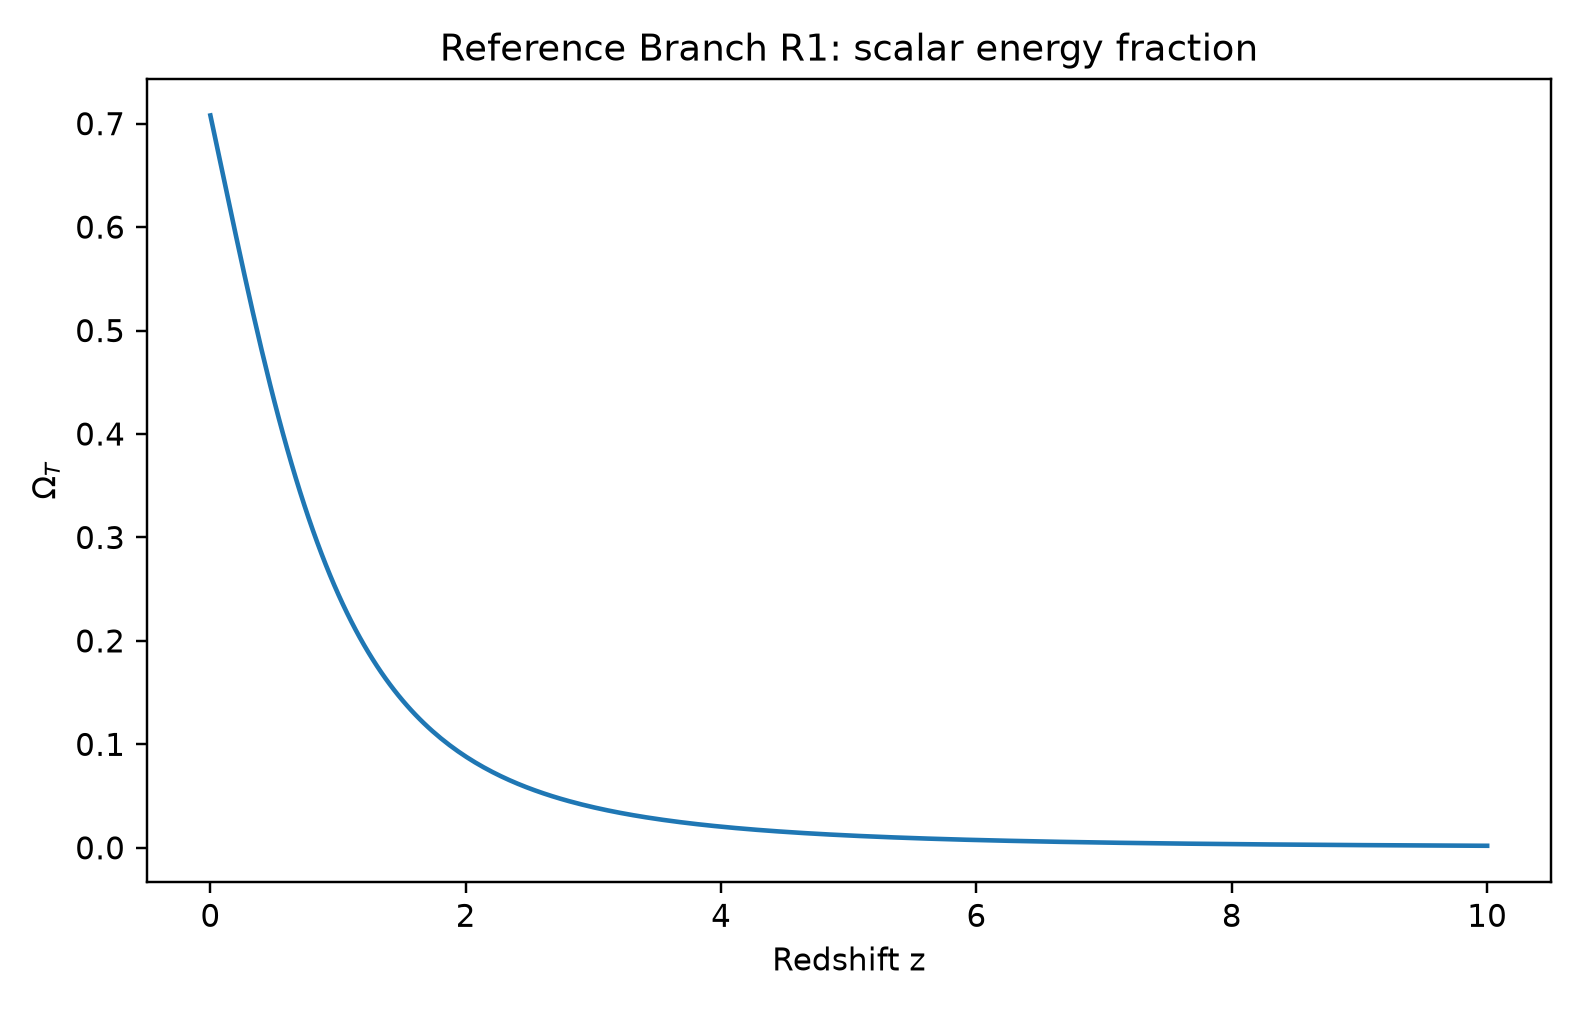
\includegraphics[width=0.82\linewidth]{figures/r1_omegaT.png}\\[0.5em]
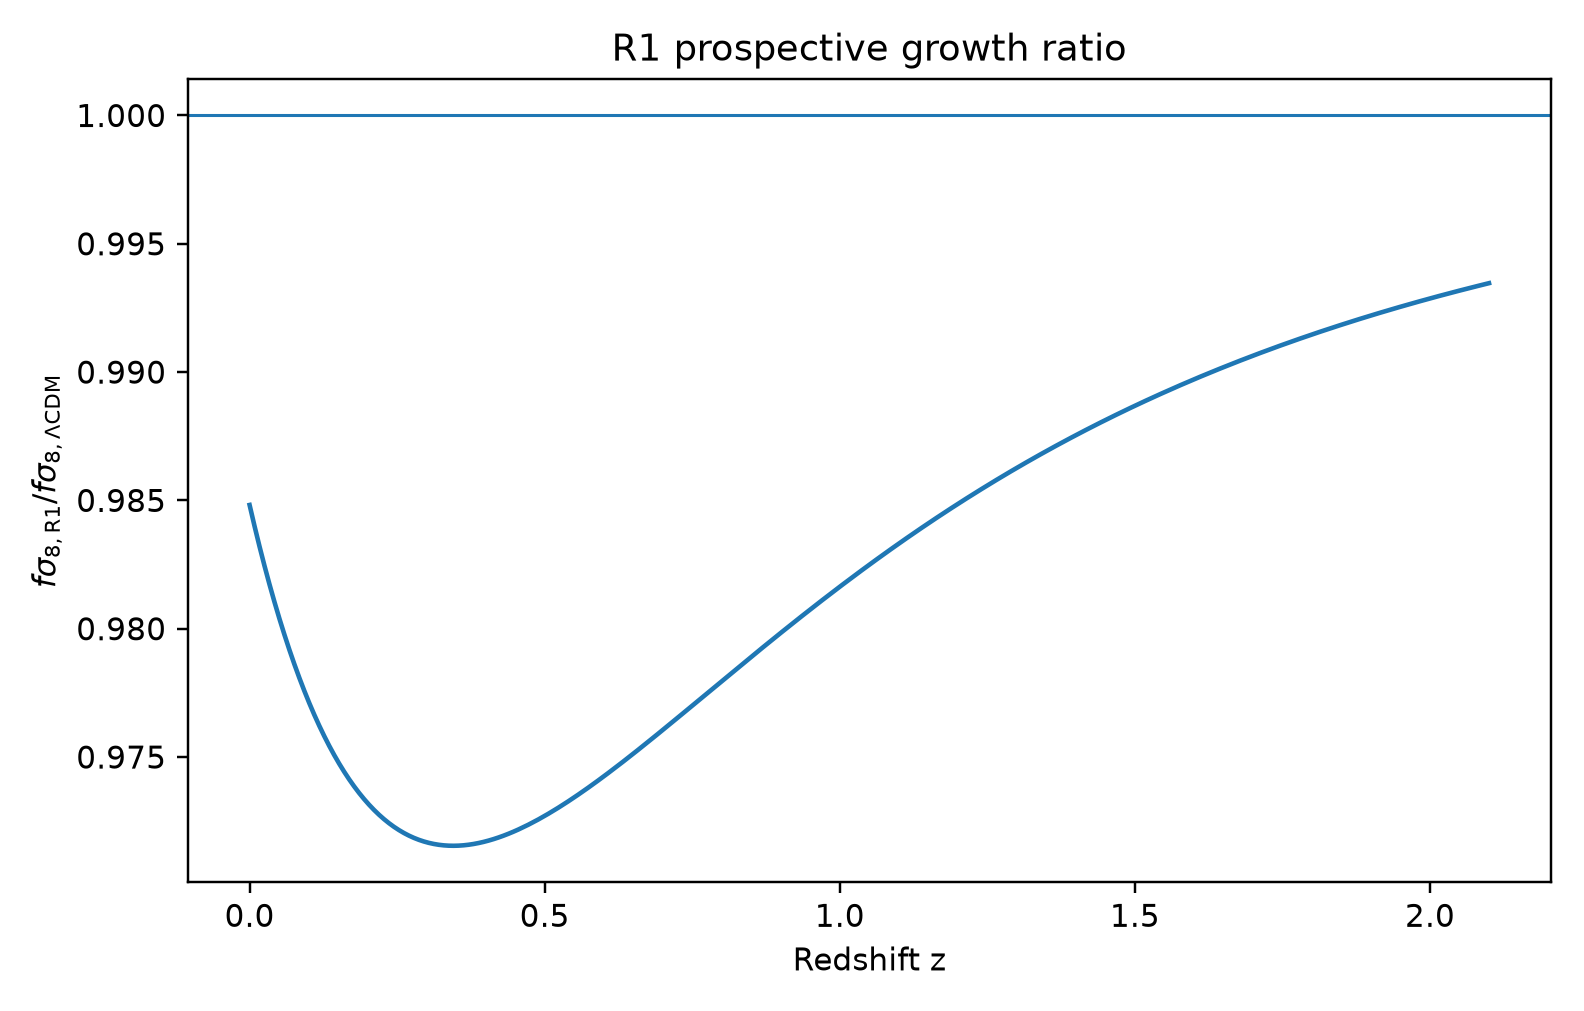
\includegraphics[width=0.82\linewidth]{figures/r1_growth_ratio.png}
\caption{Conditional frozen R1 background: scalar energy fraction (top) and growth ratio (bottom), relative to matched curved $\Lambda$CDM with identical early normalization. These are reference calculations, not fits or survey-window RSD likelihoods. Near-standard high-$n$ recovery is conditional on the illustrative retained filter.}
\label{fig:r1-background-growth}
\end{figure}

\subsection{Audited action-native quadratic stability}
Figure~\ref{fig:r1-background-growth} collects the background and reference
growth curves; Figure~\ref{fig:r1-principal-stability} shows the separate
coupled stability diagnostics.
The minimally coupled ideal dust--radiation action is reduced with the
lapse/shift Schur complement. In the retained numerical audit on
$0\le z\le2.1$, its reduced kinetic matrix is positive; the extension
through $n=1280$ has minimum eigenvalue $1.21879873\times10^{-8}$.
The principal-symbol extrapolation gives positive propagating speed
squares, with radiation approaching $1/3$ and the non-radiation branch
bounded below by approximately $0.910373$ at the sampled epochs.
The positive normalized growth tail decreases as the harmonic sequence is
extended. No ghost or high-$k$ scalar gradient instability is detected in
this audited linear/quadratic domain. These numerical checks are not a
proof of nonlinear-fluid stability, a microscopic normalization, or an
ultraviolet completion. The detailed dispersion audit is retained in
the appendix; the gravity--scalar reference kernels above remain distinct.

\begin{figure}[p]
\centering
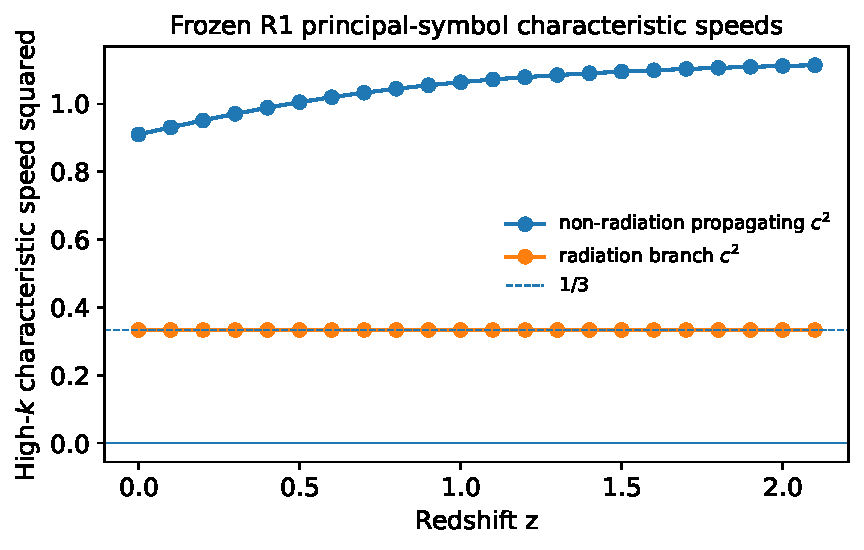
\includegraphics[width=0.82\linewidth]{figures/r1_principal_characteristic_speeds.pdf}\\[0.5em]
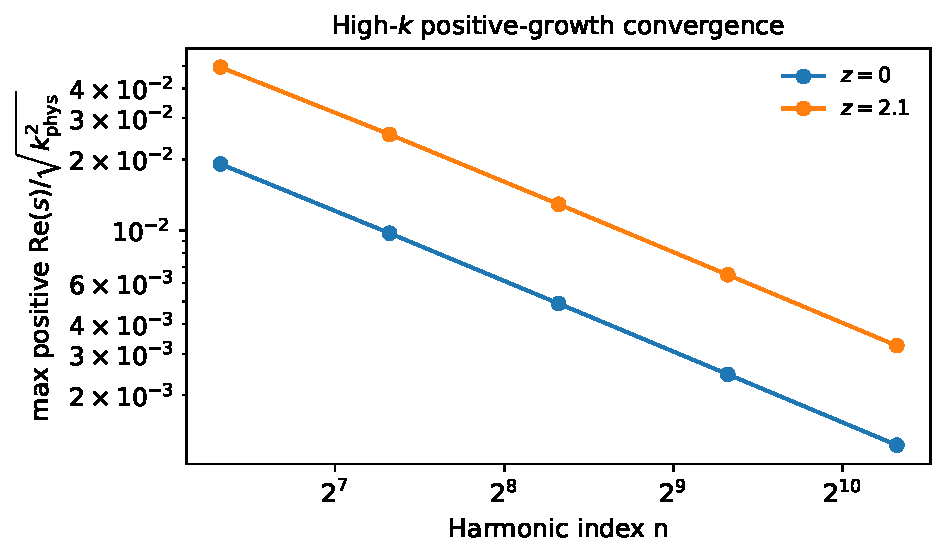
\includegraphics[width=0.82\linewidth]{figures/r1_highk_growth_convergence.pdf}
\caption{Frozen R1 coupled principal-symbol audit. Top: extrapolated characteristic speed squares at the audited redshifts, including the radiation $1/3$ reference. Bottom: the positive normalized growth tail at the two redshift endpoints decreases across the retained high-$n$ sequence. A positive finite-$n$ tail is not erased; convergence is numerical evidence within the audited quadratic domain, not an all-scale stability theorem.}
\label{fig:r1-principal-stability}
\end{figure}

\clearpage
\section{Prospective Reference-Branch Figures}

\begin{figure}[!ht]
\centering
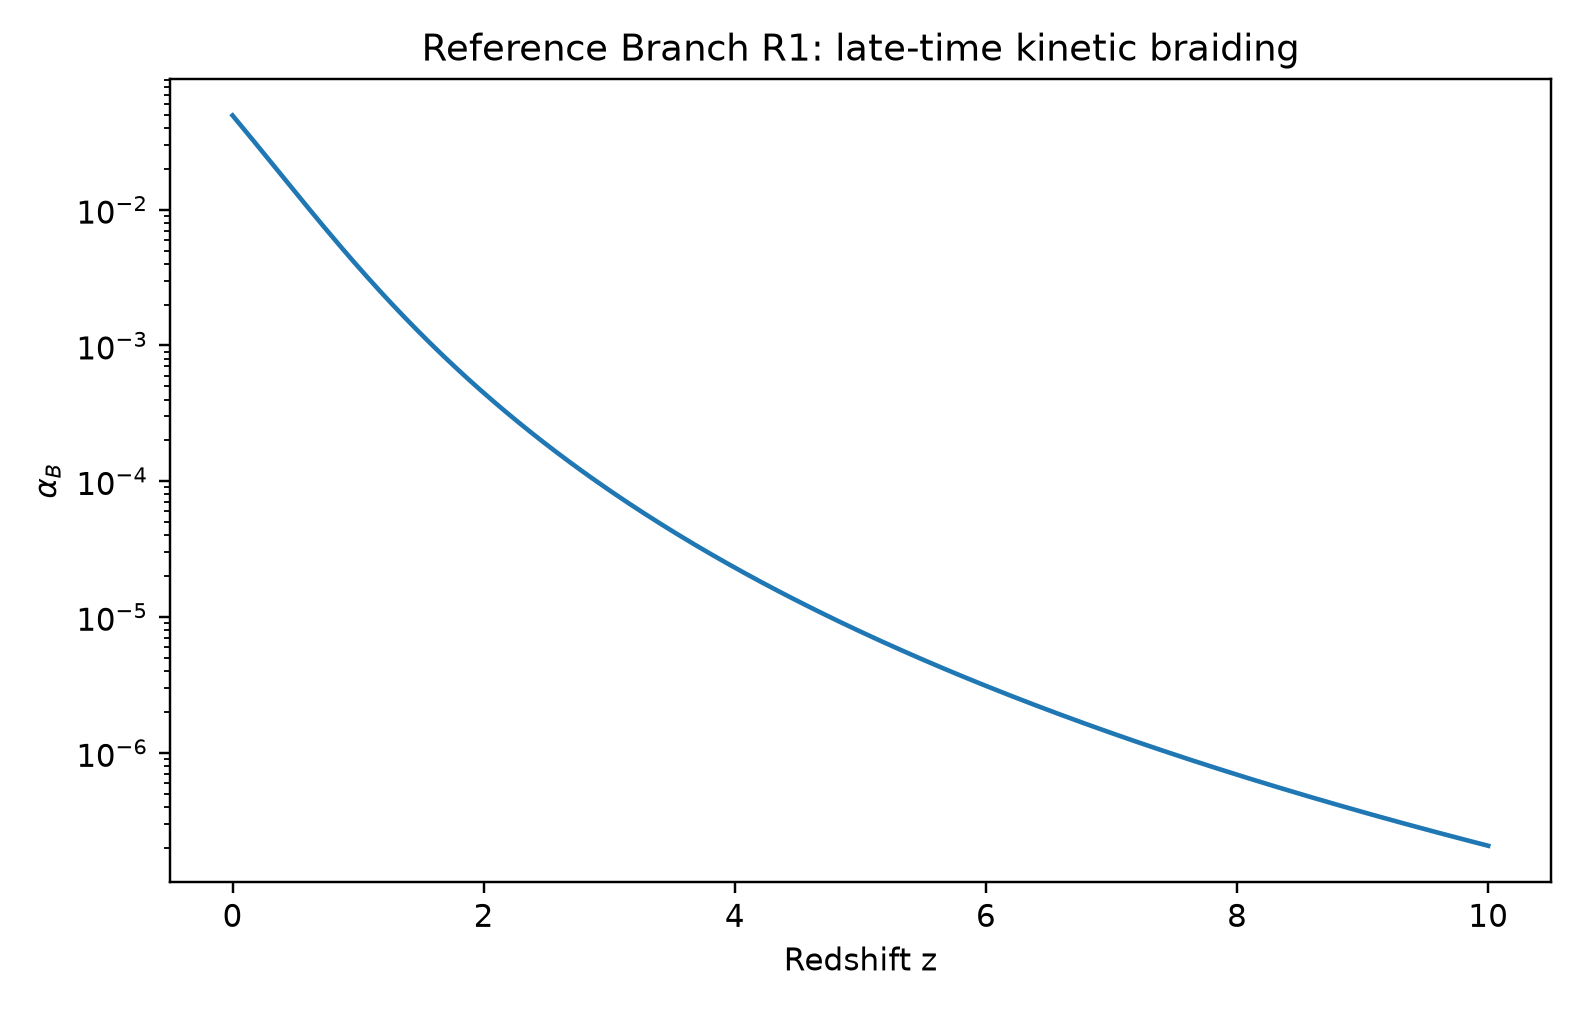
\includegraphics[width=0.68\linewidth]{figures/r1_alphaB.png}
\caption{Conditional reference calculation, not an observational fit: kinetic-braiding function \(\alpha_B(z)\) for Reference Branch R1. The logarithmic vertical scale emphasizes the suppression of the braiding sector toward high redshift.}
\label{fig:r1alphab}
\end{figure}


\begin{figure}[!ht]
\centering
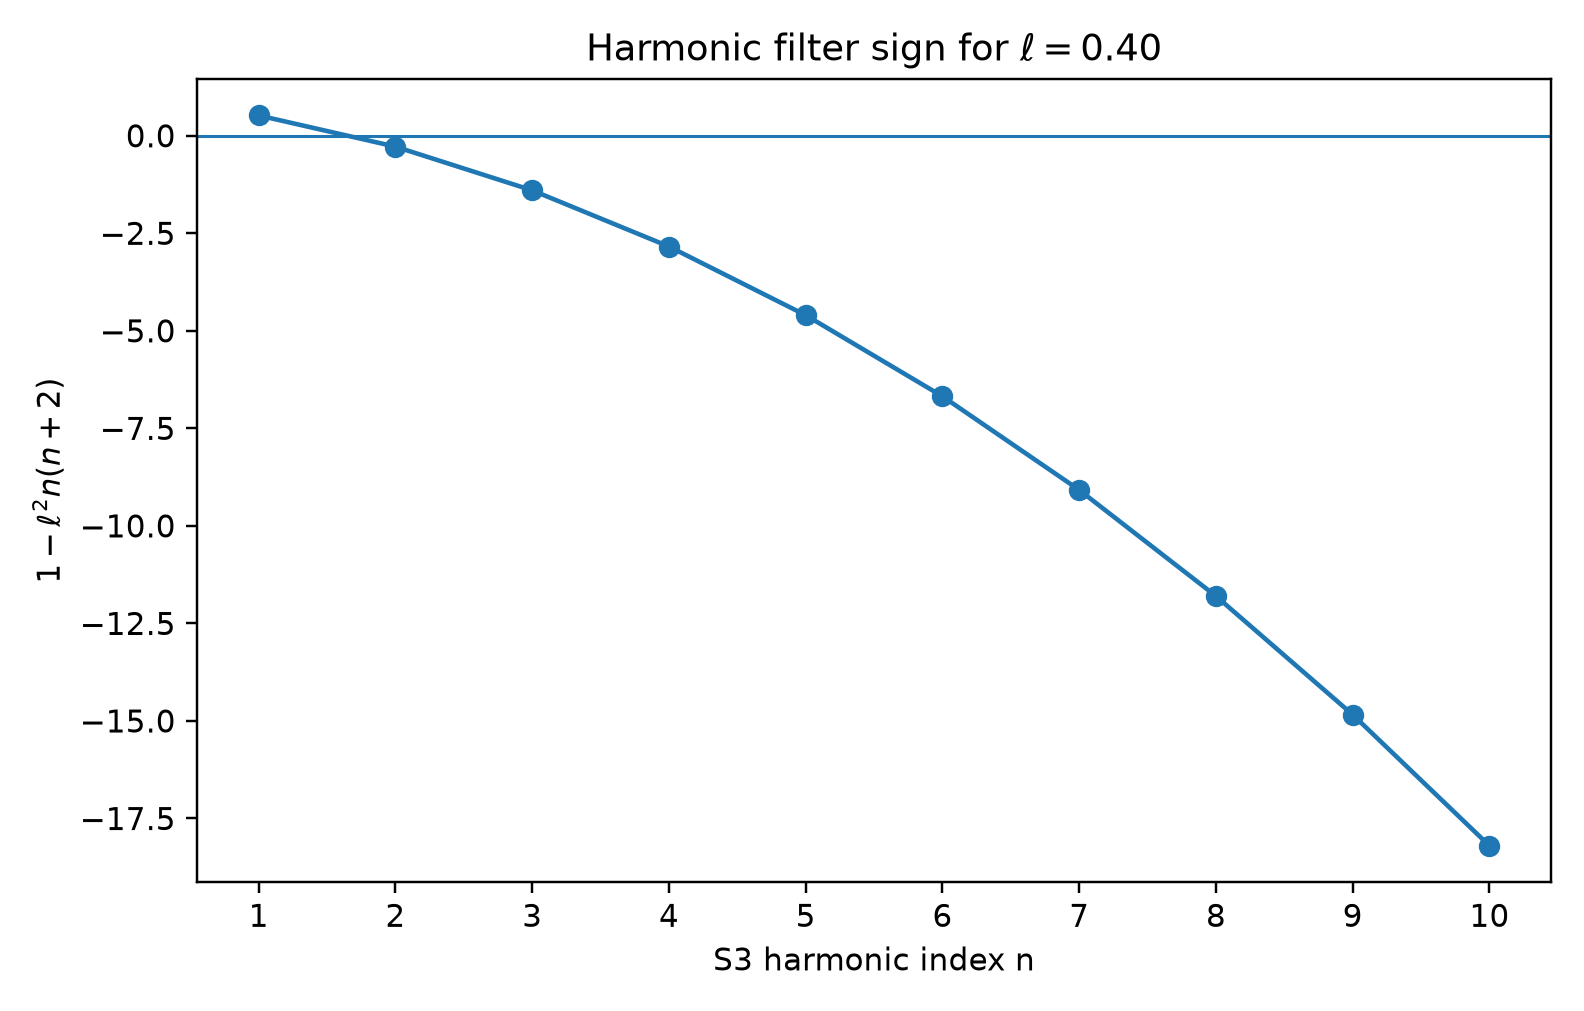
\includegraphics[width=0.68\linewidth]{figures/harmonic_filter.png}
\caption{Sign of the Schur-response factor \(1-\ell^2 n(n+2)\) for the illustrative filtering value \(\ell=0.32\), matching the canonical code. The physical \(n=2\) branch is softened and \(n\ge3\) stiffened; the displayed \(n=1\) coefficient is exceptional and excluded from propagation.}
\label{fig:harmonicfilter}
\end{figure}

\section{Discussion}

The closed-FLRW gauge audit produces a concrete correction. The first nonconstant scalar harmonic in our original notation, \(n=1\), maps to the exceptional \(N=2\) sector of standard closed-universe perturbation theory. Its scalar-derived trace-free tensor harmonic vanishes, and the regular generally covariant one-field scalar sector contains no propagating scalar degree of freedom there. Modern closed-inflation calculations likewise take physical scalar modes to begin at \(N\ge3\) \citep{KieferVardanyan2022,SpecognaEtAl2026}.

The natural response is to move the topographic carrier to the first physical scalar level: our \(n=2\), equivalent to \(N=3\). A degree-two harmonic on \(S^3\) is a traceless quadratic form in the \(\mathbb R^4\) embedding coordinates. Its cross components \(A_{4i}\) generate an exact observer-sky dipole
\[
T_{2,\rm dip}\propto\sin2\psi\,(\hat{\mathbf n}\!\cdot\!\hat{\mathbf p})
\]
without requiring a sky quadrupole.

The reduced-response filter also adapts naturally. The corrected window
\[
\frac1{15}<\ell^2<\frac18
\]
softens \(n=2\) while stiffening every higher propagating scalar harmonic \(n\ge3\). The formal \(n=1\) coefficient is irrelevant to the regular physical scalar spectrum. The enhanced carrier is therefore the first physical compact-space scalar mode.

The role of BHSM remains structural rather than a completed microscopic derivation. The imported element is the constraint-reduced response logic. The specific mixed block and the source law \(S_2\) remain exploratory until derived from the parent boundary action.

The complete \(n=2\) scalar--metric transfer kernel must still be derived in the closed cubic-Galileon background. \(D_{\rm kin}>0\) remains an inherited kinetic diagnostic rather than a complete closed-background stability proof. R1 values \(q=3\) and \(\lambda=1\) remain reference choices, and the frozen curvature forecast must not be retuned to observational results.

The R1 numerical background and high-\(n\) growth forecast do not depend on this harmonic correction. Their frozen manifest is therefore preserved unchanged, while the theoretical amendment is recorded separately before comparison with the targeted independent datasets.

\section{Conclusions}

The closed-FLRW gauge analysis resolves the principal ambiguity in the original bridge construction. Our \(n=1\) scalar harmonic maps to the exceptional \(N=2\) sector and is not retained as the ordinary propagating scalar carrier. The first physical scalar level is
\[
\boxed{n_\star=2}\qquad(\boxed{N_\star=3}).
\]
This first physical harmonic contains an exact sky-dipole subspace,
\[
T_{2,\rm dip}=A\sin[2\psi(z)](\hat{\mathbf n}\!\cdot\!\hat{\mathbf p}),
\]
when only the cross components \(A_{4i}\) are populated.

The corrected selective-response window is
\[
\boxed{\frac1{15}<\ell^2<\frac18},
\]
within which \(n=2\) is softened and every higher propagating mode \(n\ge3\) is stiffened. The next-level source-normalized response obeys
\[
\left|\frac{T_3/S_3}{T_2/S_2}\right|=\frac{8C_2}{15C_3}<\frac8{15}.
\]
The carried-forward supernova amplitude now calibrates the physical \(n=2\) dipole response. The R1 background and high-\(n\) growth predictions remain unchanged.

The revised signature is therefore
\[
\boxed{
\begin{gathered}
\text{first physical }S^3\text{ scalar mode }(n=2)\text{ enhanced}\\
\oplus\ \text{fixed-axis dipole subspace with }\sin2\psi\text{ envelope}\\
\oplus\ \text{suppressed }n\ge3\text{ susceptibility}\\
\oplus\ \text{near-GR high-}k\text{ growth}.
\end{gathered}}
\]
The next calculation is the full gauge-invariant \(n=2\) scalar--metric transfer matrix in the closed cubic-Galileon background.


\bibliographystyle{unsrtnat}
\bibliography{references}
\end{document}
